% Part 1: Estimate the linear vector field that was used to generate the points x1 from the points x0.
% Part 2: Solve the linear system and compute the mean squared error.
% Part 3: Choose the initial point (10, 10) and solve the system.
% Part 3: Visualize the trajectory as well as the phase portrait.

For this task, we are given two linear vectorfield datasets with 1000 points each. Each row represents a data point, providing the initial position $x_0^{(k)}$ and the corresponding final position $x_1^{(k)}$. The given datasets are plotted in figure \ref{fig:task2data}.

    \begin{figure}[H]
        \centering
        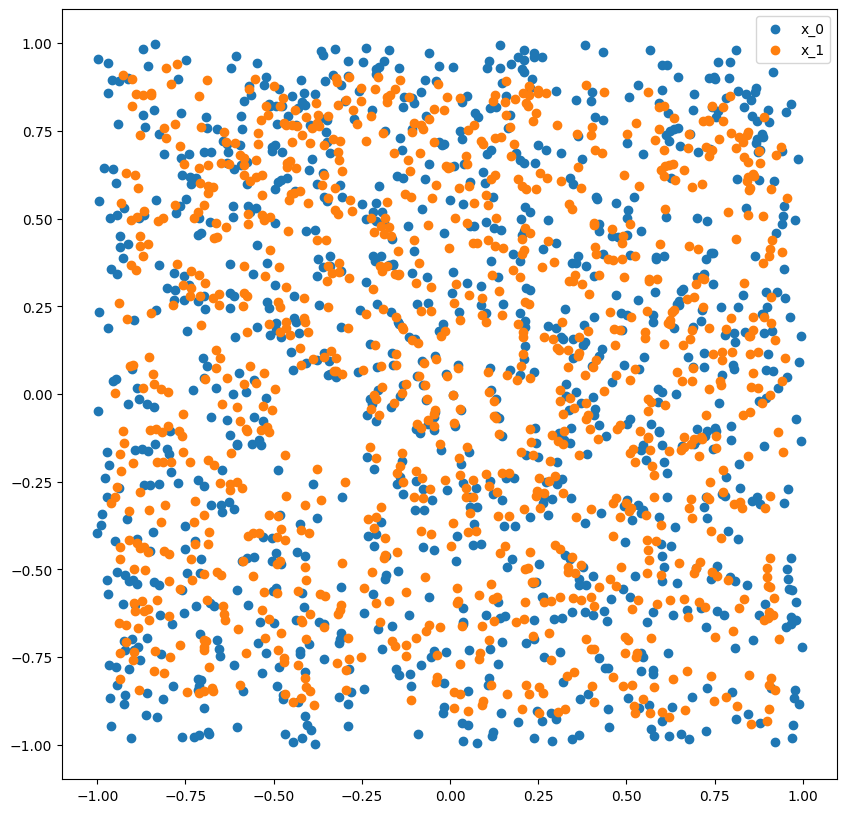
\includegraphics[width=0.5\linewidth]{images/Ex5task2_data.png}
        \caption{Dataset for task 2}
        \label{fig:task2data}
    \end{figure}

\begin{itemize}
    \item \textbf{Part 1:} For this task, we have to estimate the linear vector field that was used to generate the points {$x_1$} from the points {$x_0$}. Using the finite difference formula with a time step ($\Delta$t=0.1), the vector v\_hat is estimated at each point x$_0^{(k)}$. This captures the rate of change in the system. We then employed the least square solution to approximate the matrix A. This matrix captures the linear transformation between the initial positions and the final vectors.

    \item \textbf{Part 2:} For this task, we have to estimate the linear vector field and evaluate the accuracy of our estimated matrix A. We used the \texttt{solve\_ivp} function to simulate the linear system for each initial point $x^{(k)}_0$ up to the specified end time T$_{end}$ = $\Delta$t = 0.1. We obtained a mean squared error of \texttt{0.0030599} providing a measure of the average integration error. The approximated data after $\Delta{t}=0.1$ is shown in figure \ref{fig:task2data01}.
    
    \begin{figure}[H]
        \centering
        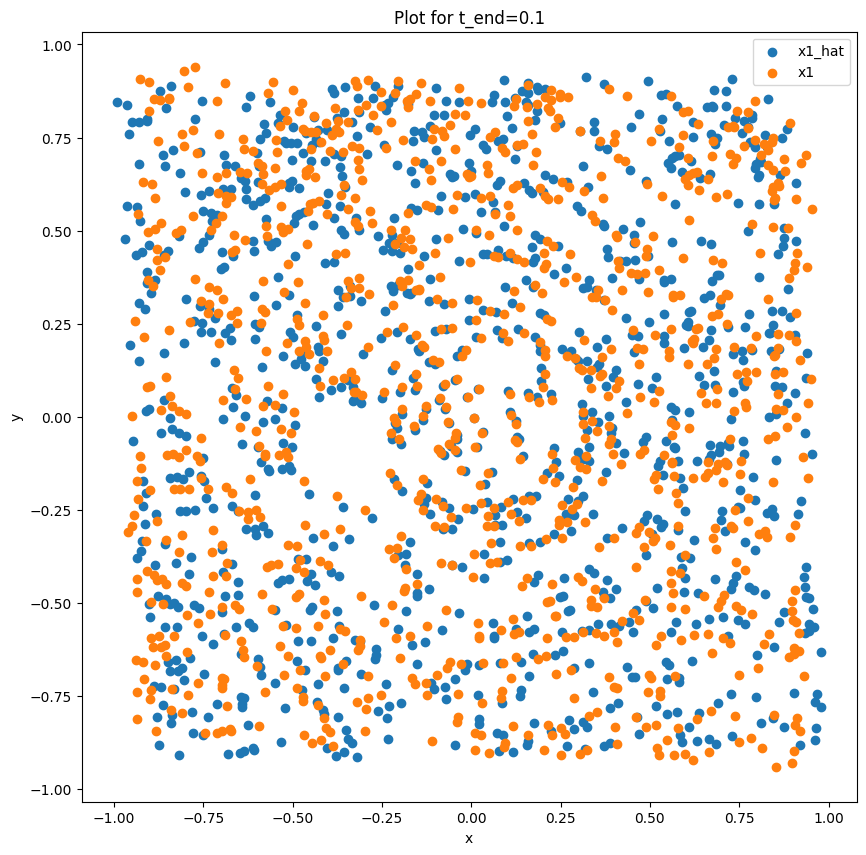
\includegraphics[width=0.6\linewidth]{images/Ex5task2_01.png}
        \caption{Approximated data after $\Delta{t}=0.1$}
        \label{fig:task2data01}
    \end{figure}

    \item \textbf{Part 3:} For this task, we first plot the phase portrait of our system and we can see that all values converge to the origin, or in other words we can say that this is the steady point of the system.\\
    We then choose an initial point (10,10), which is far outside our initial data, and solve the linear system with our approximated matrix $A\_approximated$ for a large time T$_{end}=100$. We can see that point follows the phase portrait of our system and converges to the steady point at origin.\\
    The phase portrait along with the trajectory can be seen in figure \ref{fig:task2final}.

    \begin{figure}[H]
        \centering
        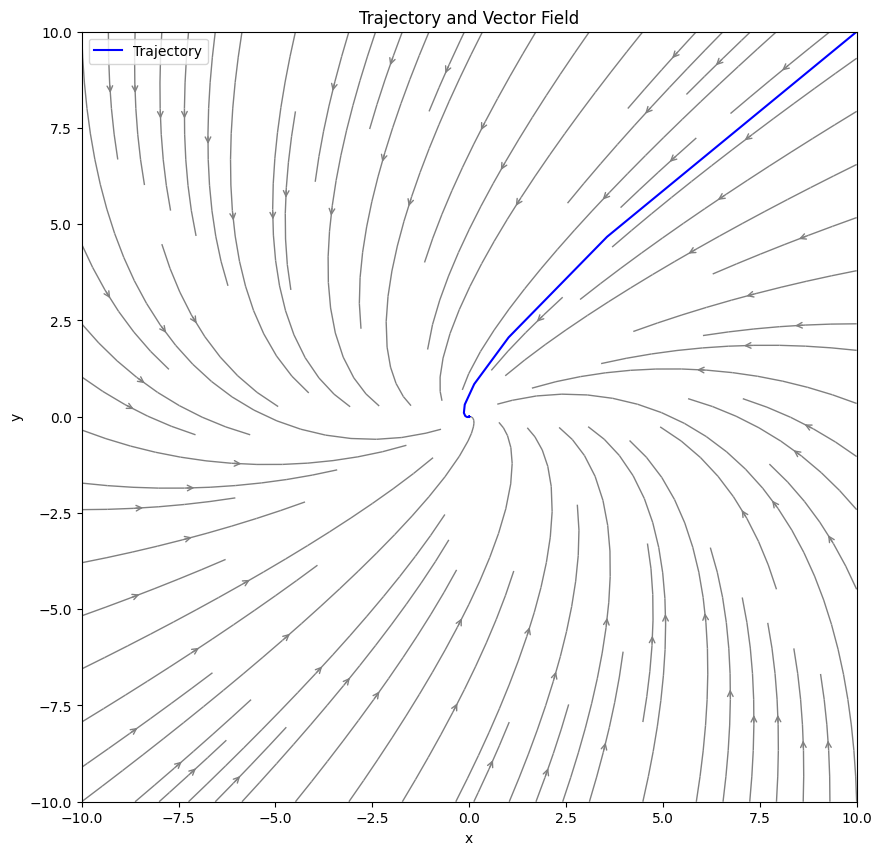
\includegraphics[width=0.6\linewidth]{images/Ex5task2_final.png}
        \caption{Plotted trajectory for $T_{end}=100$ and initial point [10,10]}
        \label{fig:task2final}
    \end{figure}
\end{itemize}